% This is "sig-alternate.tex" V1.9 April 2009
% This file should be compiled with V2.4 of "sig-alternate.cls" April 2009
%
% This example file demonstrates the use of the 'sig-alternate.cls'
% V2.4 LaTeX2e document class file. It is for those submitting
% articles to ACM Conference Proceedings WHO DO NOT WISH TO
% STRICTLY ADHERE TO THE SIGS (PUBS-BOARD-ENDORSED) STYLE.
% The 'sig-alternate.cls' file will produce a similar-looking,
% albeit, 'tighter' paper resulting in, invariably, fewer pages.
%
% ----------------------------------------------------------------------------------------------------------------
% This .tex file (and associated .cls V2.4) produces:
%       1) The Permission Statement
%       2) The Conference (location) Info information
%       3) The Copyright Line with ACM data
%       4) NO page numbers
%
% as against the acm_proc_article-sp.cls file which
% DOES NOT produce 1) thru' 3) above.
%
% Using 'sig-alternate.cls' you have control, however, from within
% the source .tex file, over both the CopyrightYear
% (defaulted to 200X) and the ACM Copyright Data
% (defaulted to X-XXXXX-XX-X/XX/XX).
% e.g.
% \CopyrightYear{2007} will cause 2007 to appear in the copyright line.
% \crdata{0-12345-67-8/90/12} will cause 0-12345-67-8/90/12 to appear in the copyright line.
%
% ---------------------------------------------------------------------------------------------------------------
% This .tex source is an example which *does* use
% the .bib file (from which the .bbl file % is produced).
% REMEMBER HOWEVER: After having produced the .bbl file,
% and prior to final submission, you *NEED* to 'insert'
% your .bbl file into your source .tex file so as to provide
% ONE 'self-contained' source file.
%
% ================= IF YOU HAVE QUESTIONS =======================
% Questions regarding the SIGS styles, SIGS policies and
% procedures, Conferences etc. should be sent to
% Adrienne Griscti (griscti@acm.org)
%
% Technical questions _only_ to
% Gerald Murray (murray@hq.acm.org)
% ===============================================================
%
% For tracking purposes - this is V1.9 - April 2009

\documentclass{sig-alternate}
\usepackage{color}
\usepackage{listings}
\usepackage{url}
\usepackage{algorithm}
\usepackage{algorithmic}
\usepackage{multirow}
\usepackage{booktabs}
\newcommand{\FIXME}[1]{{\color{red}\{FIXME #1\}}}
\newcommand{\INDSTATE}[1][1]{\STATE\hspace{#1\algorithmicindent}}
\newcommand{\EcoSim}{\texttt{EcoSim~}}
\urldef\ecosimPath\path{http://ecosimulation.com}

\newenvironment{snippet}{\begin{algorithmic}[1]}{\end{algorithmic}}

\begin{document}
%
% --- Author Metadata here ---
\conferenceinfo{SIGCSE}{2012 Raleigh, NC, USA}
%\CopyrightYear{2007} % Allows default copyright year (20XX) to be over-ridden - IF NEED BE.
%\crdata{0-12345-67-8/90/01}  % Allows default copyright data (0-89791-88-6/97/05) to be over-ridden - IF NEED BE.
% --- End of Author Metadata ---

\title{Parallel Programming in Elementary School}
%
% You need the command \numberofauthors to handle the 'placement
% and alignment' of the authors beneath the title.
%
% For aesthetic reasons, we recommend 'three authors at a time'
% i.e. three 'name/affiliation blocks' be placed beneath the title.
%
% NOTE: You are NOT restricted in how many 'rows' of
% "name/affiliations" may appear. We just ask that you restrict
% the number of 'columns' to three.
%
% Because of the available 'opening page real-estate'
% we ask you to refrain from putting more than six authors
% (two rows with three columns) beneath the article title.
% More than six makes the first-page appear very cluttered indeed.
%
% Use the \alignauthor commands to handle the names
% and affiliations for an 'aesthetic maximum' of six authors.
% Add names, affiliations, addresses for
% the seventh etc. author(s) as the argument for the
% \additionalauthors command.
% These 'additional authors' will be output/set for you
% without further effort on your part as the last section in
% the body of your article BEFORE References or any Appendices.

\numberofauthors{4} %  in this sample file, there are a *total*
% of EIGHT authors. SIX appear on the 'first-page' (for formatting
% reasons) and the remaining two appear in the \additionalauthors section.
%
\author{
% You can go ahead and credit any number of authors here,
% e.g. one 'row of three' or two rows (consisting of one row of three
% and a second row of one, two or three).
%
% The command \alignauthor (no curly braces needed) should
% precede each author name, affiliation/snail-mail address and
% e-mail address. Additionally, tag each line of
% affiliation/address with \affaddr, and tag the
% e-mail address with \email.
%
% 1st. author
\alignauthor
Chris Gregg\\
       \affaddr{University of Virginia}\\
       \affaddr{Department of Computer Science}\\
       \affaddr{Charlottesville, VA}\\
% 2nd. author
\alignauthor
Luther Tychonievich\\
       \affaddr{University of Virginia}\\
       \affaddr{Department of Computer Science}\\
       \affaddr{Charlottesville, VA}\\
% 3rd. author
\alignauthor Kim Hazelwood\\
       \affaddr{University of Virginia}\\
       \affaddr{Department of Computer Science}\\
       \affaddr{Charlottesville, VA}\\
\and  % use '\and' if you need 'another row' of author names
% 4th. author
\alignauthor James Cohoon\\
       \affaddr{University of Virginia}\\
       \affaddr{Department of Computer Science}\\
       \affaddr{Charlottesville, VA}\\
}
% There's nothing stopping you putting the seventh, eighth, etc.
% author on the opening page (as the 'third row') but we ask,
% for aesthetic reasons that you place these 'additional authors'
% in the \additional authors block, viz.
%\date{30 July 1999}
% Just remember to make sure that the TOTAL number of authors
% is the number that will appear on the first page PLUS the
% number that will appear in the \additionalauthors section.

\maketitle
\begin{abstract}
Traditional introductory programming classes focus on teaching sequential programming
skills using conventional programming languages and single-threaded applications.
It isn't generally until much later in a student's programming education that he or she learns
about parallel programming and associated topics such as race conditions, locks, or data
consistency.  With the increased popularity of 
multicore CPUs and GPUs capable of GPGPU computing, there is a greater 
need for programmers who are not only proficient in parallel programming, but who are
not burdened by an inclination towards trying to solve a problem in a sequential fashion, with
parallelism tacked on as an afterthought.

Pedagogically, there is a case to be made that teaching parallelism first is an important 
step towards educating tomorrow's programmers for the challenges of programming multicore and GPGPU
systems.  We present an overview of a five-day introductory parallel programming course we 
taught to a group of nine and ten year-olds, using a near-natural language syntax
parallel programming language we created, targeted towards students with no previous programming
experience.  Our language is simple but powerful and consists 
of a simulated parallel programming environment and the ability to run or step through programs.

We provide examples of student-written code that demonstrates their understanding of some basic
parallel programming concepts, and we describe the overall course goal and specific lesson plans
geared towards teaching students how to ``think parallel.''
\end{abstract}

% A category with the (minimum) three required fields
\category{H.4}{Information Systems Applications}{Miscellaneous}
%A category including the fourth, optional field follows...
\category{D.2.8}{Software Engineering}{Metrics}[complexity measures, performance measures]

\terms{Languages, Design}

\keywords{Concurrent, distributed, and parallel languages, Instructional Design,
Introductory Programming, Pedagogy, Education}

\section{Introduction}
Introductory programming classes are almost universally taught 
using languages designed primarily for single-threaded applications.  Multi-threaded or
parallel programming concepts are considered advanced, and it is rare that students learn about
parallel programming before a second or third programming course.  Indeed, most colleges and
universities in the United States provide a single parallel programming course available 
to upper level undergraduates or graduate students\FIXME{citestats}, and such courses are
almost always optional in the computer science curriculum.  In many cases, only students who
are interested in high performance computing are ever exposed to parallel programming, and the
average programmer never receives any traditional instruction in parallel programming at all.
Additionally, when students do learn parallel programming, many have difficulties transitioning
from a sequential-programming mentality to a parallel programming mentality, especially as parallel
programming is considered ``hard'' by many students and instructors 
alike.~\cite{parallelExpectations}

Within the last five years, multicore computing has become the \emph{de facto} standard on
desktops and laptops, and General Purpose GPU (GPGPU) computing has matured such that multi-core 
GPUs can be programmed with minimal extensions to traditional languages such as C++ and 
Python~\cite{gpgpuLanguages}.  The trend towards increasing cores to program on a
single machine does not show any signs of abating in the near future~\cite{multicoreTrends}, and
therefore parallel programming skills are going to become increasingly important.  Programmers
must not only thoroughly understand parallel programming concepts such as race conditions,
atomicity, synchronization, and deadlock, but they must be able to look at a computing problem
and think of solutions that utilize parallel processes.

With the disconnect between sequential-only introductory programming classes and the necessity for
programming students to learn parallel programming concepts and methods in mind, we developed
an introductory parallel programming course that specifically targeted novice programmers.  We
designed a language, called \emph{EcoSim}\footnote{\emph{EcoSim} is so-named because the original 
class we taught with it focused on an \emph{eco}logical \emph{sim}ulation.}\FIXME{Are we going to 
name the language officially?}, that simulates a parallel programming environment and has a highly
accessible natural language syntax.  Programs written in \emph{EcoSim} have the ability to exhibit race 
conditions, allow both atomic and non-atomic variable assignment, and show increased performance
when the number of cores is increased.  It is a turing-complete language, and
contains a number of basic functions geared towards making the programs interesting for novice
programmers.  Figure \ref{fig:exampleProgram} shows an example \emph{EcoSim} program that defines and
draws ten green ``plants'' on the screen, where the plants are represented by circles of radius 10.
Figure \ref{fig:ecosimScreencap} shows the \emph{EcoSim} development environment, which includes
a code window, settings, a console window with output messages, and a window for graphical
objects.
\begin{figure}
\begin{algorithmic}[1]
%\INDSTATE[x]{code} indents x number of tabs, \INDSTATE{code} indents a single tab
\STATE{a plant has}
  \INDSTATE{a position}
  \INDSTATE{size, a number}
  \INDSTATE{a color}
\STATE{}
\STATE{create 10 plant and for each}
  \INDSTATE{do in order}
  \INDSTATE{replace the plant's color with green}
  \INDSTATE{replace the plant's size with 10}
\end{algorithmic} 
\caption{A simple \emph{EcoSim} program to define and create ten green ``plants'' on the screen.}
\label{fig:exampleProgram} 
\end{figure}

\begin{figure}
\centerline{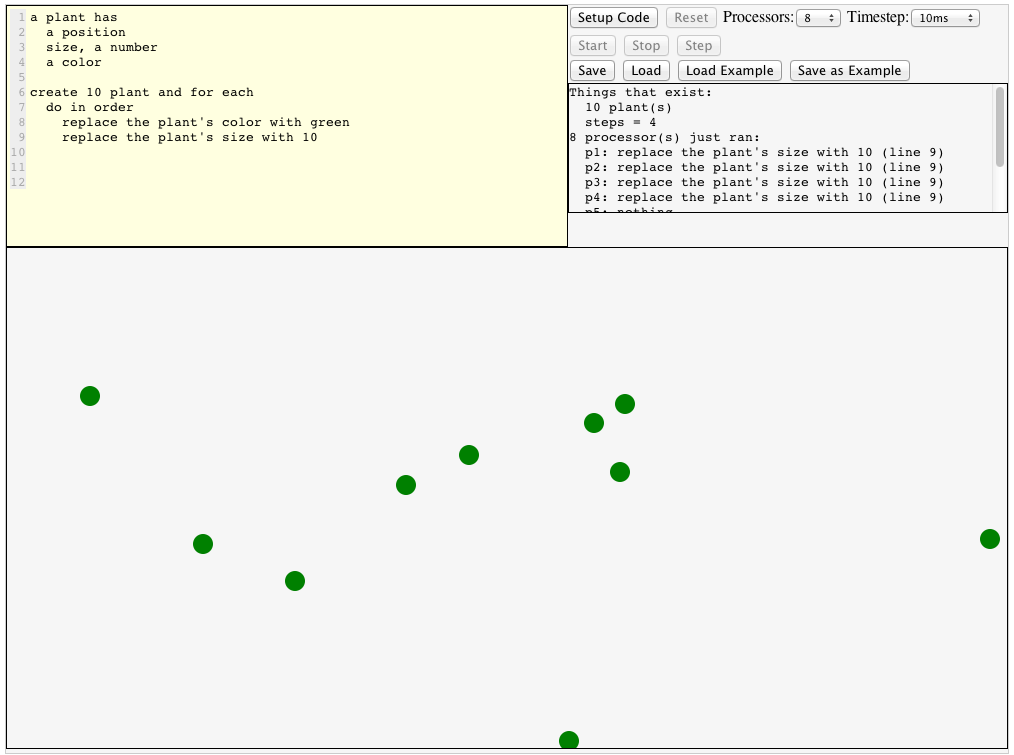
\includegraphics[width=.49\textwidth]{figures/EcosimScreencap.png}}
\caption{The \emph{EcoSim} web-based integrated development environment hosted at
\ecosimPath{}.  Code is written and debugged in the top left window, settings are on
the top right, a console with runtime and debug information is below the settings, and the
main window shows the graphical output of the program.}
\label{fig:ecosimScreencap}
\end{figure}

We had three overarching goals in mind for the course we designed around \emph{EcoSim}:
\begin{enumerate}
\item Introduce the students to simple parallel programming ideas using multiple processors.
\item Provide interesting parallel programming examples the students could easily modify and
learn from.
\item Teach the students to ``think parallel'' about computing problems we gave them, or that
they thought up on their own.
\FIXME{should we include the define the task/describe a solution/tell the computer here?}
\end{enumerate}

We presented the course, titled, ``Programming the Computers of the Future'' to two classes of 
eighteen 4th and 5th grade (9 and 10 year old) students during a five-day enrichment program.
Each class period was two hours long, and the students had a week between classes, although they
could access the programming development environment online to continue learning independently.
None of the students had significant prior programming experience.
We based the course curriculum on creating a simulated ecosystem, starting with simple objects
such as stationary plants that could grow in place, and eventually creating herbivores and
carnivores that could move about the screen.
Our lessons included group exercises that introduced parallel programming concepts and general
programming-style problem solving, and each lesson included example \emph{EcoSim} programs with
time for the students to modify or attempt to create new programs on their own.

We had many successes in our pilot course:

\begin{enumerate}
\item Exit surveys collected from the students in both classes showed enthusiastic responses to the
class, and students reported that they learned a number of programming concepts.
\item Student code examples show that by the end of the class students were familiar with the
language and were able to write programs that took advantage of parallel concepts.
\item After one or two classes the students
felt comfortable with basic concepts of \emph{EcoSim} and were able to write rudimentary
parallel programs without trouble.  By the end of the course, a number of students designed
and implemented creative programs that highlighted the parallel nature of the language.
\end{enumerate}

\section{Background and Related Work}

Parallel computing has a long history, dating back to 1955 and the IBM 704
and its ability to compute parallel arithmetic~\cite{hockney1988parallel}.  Amdahl's law,
defining the maximum possible speedup due to parallelization, was coined in 
1967~\cite{amdahl1967validity}, and multiprocessor mainframes and multinode distributed
computing platforms provided most of the world's parallel processing until the early 2000s.
However, even with multiprocessor systems, programmers were first taught how to write
sequential applications, generally learning parallel programming concepts for specific
computers or platforms.  The microcomputer explosion of the late 70s and early 80s
ensured that most programmers were exposed to uniprocessor machines as their first computers,
and thus their first programming experiences were with sequential programming languages as well.
Today, multicore desktop and laptop computers are ubiquitous, and in order to make the most
efficient use of these computers, parallel programming is necessary.  Furthermore, when novice
programmers sit down to write their first code, it is using a a parallel computer.

There are numerous programming languages available for desktop parallel programming.  Many of
these languages are extensions, libraries, or APIs built on top of sequential languages such 
as C or Fortran (e.g., OpenMP, CUDA, 
OpenCL, Intel Thread Building Blocks, pthreads, Cilk,
Co-array Fortran, and Unified Parallel C),
requiring a novice programmer to first become proficient in a sequential language before
tackling the parallel programming concepts.  While this does not necessarily hinder a student's
overall programming ability, parallel programming tends to receive less importance than simply
learning the sequential aspects of the language.  There have been a number of studies on teaching 
parallel programming concepts using traditional languages at the 
undergraduate level~\cite{freshmanParallel,undergraduateParallel,gridPortal} 
and at least one at the secondary school level~\cite{highSchoolParallel}.

There are also languages designed for parallel programming, but they tend have advanced
syntax and be targeted towards
students already proficient at programming in general (e.g., X10\cite{X10}, 
NESL~\cite{nesl-impl-94}, and Go~\cite{GoLanguage}).  It would be hard to suggest any of these
languages to an absolute beginner programmer.


\section{EcoSim: An Introductory Parallel Programming Language}
To teach programming, it is necessary to select a language or environment.
We had a number of constraints on the language we taught:
\begin{itemize}
	\item It should be fundamentally parallel.
	\item The meaning of programs should require little explanation.
	\item It should run without installation.
\end{itemize}
Since we were aware of no language having all of these characteristics, we designed one.
To make it run without installation, we implemented it entirely in javascript
and wrapped it in website having a simple editor and interaction environment.
Notably absent from our goals was being a ``complete'' language;
for example, since we did expect to teach pointers, we did not include pointer mechanisms in the language.

\subsection{Themes and Mantras of EcoSim}
We wanted out language to get out of the way of teaching parallel computing principals and practice.
To facilitate this goal, we developed a set of guiding themes or mantras by which we designed the language.

First and most important, we wanted each core statement to be it's own explanation.
When considering a possible language syntax, we would ask 
``How would we explain this construct to a complete beginner? Can we replace it with that description?''
For example, we would describe the behavior of the assignment statement \texttt{x = 3}
as ``replacing the value stored in \texttt{x} with \texttt{3}'',
so we decided to write is as \texttt{replace x with 3}.

Second, we wanted to make sure students didn't loose sight of the fact that some processor must execute each statement.
We decided to realize this goal by having statement in EcoSim be written to \emph{address} a processor.
Thus, instead of the OO-style \texttt{gen.nextInt()} we preferred 
\texttt{get the next number from gen} or \texttt{gen's next number}.

Finally, we wanted to make naming values the exception instead of the rule.
In common speech we rarely name values;
instead we say things like ``the square of \emph{a number} is \emph{the number} times \emph{itself}'',
making use of common reference techniques in English.

\subsection{EcoSim Syntax \& Semantics}
EcoSim was implemented as a statically-typed interpreted language with type inference
using a modified recursive descent parser that type-checked and parsed in the same pass,
allowing some degree of context sensitivity in the language definition.
For example, consider the line \texttt{how to cow a person}
is a syntax error if ``cow'' is a type,
declares a single-parameter subroutine ``cow'' is ``person'' is a type,
and declares a parameterless subroutine ``cow a person'' if neither are types.
While this parser design allowed us to easily implement multi-word statements,
it also proved somewhat difficult to implement correctly.
We expect there are still several corner cases we failed to handle correctly.

We chose to implement blocks with Python-like indentation.
This turned out to be a bad idea, and caused the students considerable difficulty.
Upon reflection, spoken English does not really have a notion of blocks;
the closest thing to blocks we know of in natural language is bulleted lists,
which are not straightforward to represent and nest in plain text.

We had found in our contact with other CS1 courses that statements like ``$x = x + 1$'' confuse students.
To prevent this confusion, we require that if a name appears as an l-value and an r-value,
then in the r-value it must be preceded by the word ``old,'' as in
\begin{snippet}
\STATE{replace x with old x + 2}
\end{snippet}


\subsubsection{(Nearly) Standard OO Constructs}
Many elements of EcoSim correspond closely to common procedural/OO elements:
\\\begin{tabular}{|l|l|}\hline
EcoSim & C-like\\\hline\hline
start x as 3 & var x = 3\\\hline
refer to x as y & alias y = x\\\hline
replace x with 3 & x = 3\\\hline
x's number & x.anonymousNumber\\\hline
x's 2nd big thing & x.bigThing[1]\\\hline
as long as 2 $<$ 3: & while (2 $<$ 3)\\\hline
\begin{tabular}{@{}l@{}}if 2 $<$ 3\\~ \dots\\otherwise\\~ \dots\end{tabular} & \begin{tabular}{@{}l@{}}if (2 $<$ 3) \\~ \dots\\ else\\~ \dots\end{tabular}\\\hline
repeat 3 times: & for (int i=0; i$<$3; ++i)\\\hline
\begin{tabular}{@{}l@{}}a plant has\\~ size, a number\\~ 2 position\end{tabular} & \begin{tabular}{@{}l@{}}struct plant \{\\~ number size;\\~ position[2] anonymousPosition;\\\}\end{tabular}\\\hline
a plant's r is 3 & plant \{ function r() \{ return 3; \} \}\\\hline
how to eat a bug & function eat(bug theBug)\\\hline
do in [any] order & \{\\\hline
\end{tabular}\\
A few of these constructs deserve slightly more discussion.

The \texttt{refer to} construct is used to give a name to something that is about to be shadowed,
and differs from \texttt{start} in that assigning to it modifies the original.
Thus 
\begin{snippet}
\STATE{start x as the position's x}
\STATE{replace x with 2}
\end{snippet}
does not change the position, whereas
\begin{snippet}
\STATE{refer to the position's x as x}
\STATE{replace x with 2}
\end{snippet}
does.

Object methods must be a single expression, and may refer to the owning object.
Once created, there is no syntactic difference between methods and member variables;
both are accessed with the \texttt{'s} operator.

The \texttt{repeat} construct is unordered and may run in parallel.
In hindsight the word ``repeat'' implies sequentiality and should probably have been ``do'' instead.

Blocks may be introduced by one of four different \texttt{do} constructs.
The principal two, \texttt{do in any order} and \texttt{do in order},
specify whether the statements within the block may be executed in parallel or not.
The other two add the word ``atomically'' (e.g., \texttt{do atomically in any order})
and causes all of the statements of the block to be executed ``at the same time''.
All blocks must be introduced with an explicit \texttt{do} statement.

\subsubsection{Unique Constructs}\label{sec:ecosim-unique}
Some parts of EcoSim have no direct parallel to any language of which we know.
One is the inability to create named objects.
Inside the EcoSim runtime is stored, for each type, a single collection of ``live'' objects of that type.
The statement
\begin{snippet}
\STATE{create 15 number}
\end{snippet}
adds 15 new elements to the runtime's collection of existing number-type objects.
The \texttt{create} statement may also initialize each newly created object:
\begin{snippet}
\STATE{create 15 number and for each}
\INDSTATE{replace the number with 7}
\end{snippet}

Since objects are not named, they can only be accessed anonymously
either via iteration or random selection.
Thus, after running the following code
\begin{snippet}
\STATE{for each number}
\INDSTATE{replace the number with the old number + 3}
\STATE{for some number}
\INDSTATE{replace the number with the old number -- 1}
\end{snippet}
every number will be incremented by 3 (in parallel)
and one number (selected at random) will be decremented by 1.

This model of creation as placing an object in a global collection
greatly simplifies the removal of objects without impacting other processors that may be using it.
The statement
\begin{snippet}
\STATE{destroy the number}
\end{snippet}
simply removes that object from the collection;
other processors that my be operating on the object are free to do so,
but no new statements can refer to it again.
Once no references remain, the object is garbage collected.

The last unique element of EcoSim we'll discuss is the ability to talk to the processors directly.
For example, we can write
\begin{snippet}
\STATE{when bored}
\INDSTATE{create a number}
\end{snippet}
to tell every processor to spend their idle time adding more numbers to the runtime's collection.
This is also how we handle events:
\begin{snippet}
\STATE{when a sheep hits a shrub}
\INDSTATE{destroy the shrub}
\end{snippet}

\subsection{EcoSim Runtime Model}
The goal of the EcoSim runtime is to provide simple visual interaction
and to emulate a multi-processor environment
using only javascript in an ordinary web browser.
This is realized by storing global lists of types (see~\S\ref{sec:ecosim-unique}),
a lost of emulated processors, and a shared work queue.
Additionally, the runtime contains a collision detection algorithm.

EcoSim has four builtin types:
``number'', a 64-bit IEEE floating-point number;
``color'', an HTML-compliant color string;
``comparison'', or boolean, which never brought up explicitly to the students;
and ``position'', which is defined as
\begin{snippet}
\STATE{a position has}
\INDSTATE{x, a number}
\INDSTATE{y, a number}
\end{snippet}
If a type has both a ``position'' and a ``size'' (either as a field or a method)
then it is drawn every update cycle as a circle (either black or its ``color'')
and is included in the collision tracking routine.

The basic process the runtime follows each cycle is as follows:
\begin{algorithmic}[1]
\STATE{If there is work in the queue, assign it to processors}
\STATE{If there are leftover processors, check for collisions and assign the handlers to processors}
\STATE{If there are leftover processors, assign each a ``when bored'' handler}
\STATE{Update the display of what each processor is doing}
\STATE{Have each processor execute one step and put their remaining computation in the queue}
\STATE{Update the display of where the objects are}
\end{algorithmic}

\subsection{EcoSim: The Big Picture}
The EcoSim language and EcoSim runtime together provide an environment 
for introducing programming with a parallel model from the beginning.

The language is designed to be easy to read by non-programmers, 
realizing the mantra ``replace the syntax with its explanation'' 
with constructs like ``as long as x $>$ 10: replace x with old x -- 10''.
It is also designed to be fundamentally parallel and processor-aware
with all statements worded to address a processor
and any non-parallel behavior expressed explicitly using ``do in order'' and ``do atomically'' constructs.
It is also designed so that most values need not be named,
reducing the confusion of shadowed names
and allowing for a more English-like expression of ideas.

The runtime is designed to allow an easy introduction to parallel execution.
It runs on any browser with support for the HTML5 canvas element utilizing only standard javascript 1.3 constructs.
The runtime emulates an array of processors working off of a shared work queue 
and displays what work each processor is doing at each step.
The language and runtime together support event-based programming of circular objects
with collision detection and idle-time behaviors.

\FIXME{\thesubsection\ is meaningless. Destroy it? change it? Move it earlier?}

\section{Course Overview and Lesson Plans}
The pilot course we created was for fourth and fifth grade students in an enrichment program
that is run through our university.  We designed the course and \emph{EcoSim} concurrently,
and both were targeted for our audience of self-selected primary school students with no
prior formal programming experience.
\begin{enumerate}
\item Overview (ecosystem in parallel)
\item Starting to "think parallel" -- student sort
\item Ingraining the idea of multiple processors working independently to solve the same problem.
\item Constantly let kids show off what they have accomplished
\item the idea of "when bored", for some, for all
\item atomicity and race conditions (class example on board -- roll/read/roll/write)
\item St. Matthew Island
\end{enumerate}

\subsection{Ecosystem in Parallel}
The original conception of the pilot course was, simply, ``Let's teach fourth and fifth graders
about parallel programming.''  We decided on an ``ecosystem'' theme for the course, based on a
number of reasons.  First, students at this level are familiar with real-life ecosystems, and we
felt that they would find the topic interesting.  Second, ecosystems have a number of 
embarrassingly parallel characteristics; for example, in a forest there are multiple copies
of trees which can each be handled independently and in parallel.  
Finally, we knew we could model a simple ecosystem 
and then build upon the original model to make it more complex.  Starting with a forest of
stationary plants that have a single ``grow'' characteristic, we added motile herbivores that
consumed the plants.  We then added the ability for the inhabitants to reproduce and gave them
the ability to die from starvation, and then eventually we added carnivores as well.  
By the end of the course students had expanded the ecosystem to include plants that only
grew during the day, hunters, and even carnivorous and poisonous plants.  

Students quickly learned the importance of initial conditions and parameters, both from a 
computational perspective and a scientific one.  For example, students found that starting 
ten thousand herbivores in a field with only ten plants
not only slows the computer to a crawl, but the herbivores quickly decimate the plant population
and start to die from starvation.  We spent a number of classes discussing and
modeling the intriguing real-life case of a herd of reindeer who overpopulated a remote
island in Alaska and subsequently died out~\cite{klein1968introduction,stMatthewIsland}, 
and with the \emph{EcoSim} model the students could adjust the parameters to find an
equilibrium that would have allowed the reindeer to survive.

\subsection{Getting the students to ``think parallel''}
At the beginning of each class period and before writing any code, we first introduced the 
students to a parallel programming concept in a full-class discussion, usually with an activity.
For instance, on the first day of class we introduced the students to the difference in
computational time between parallel and sequential processes by having them sort themselves
by height.  First, we allowed the students to line themselves up by height, all at once (the
parallel method), and we timed this; it took roughly forty-five seconds for a class of eighteen.
Next, we re-randomized the class and assigned one student to be the ``processor,'' in charge
of sorting the students two at a time.  Unsurprisingly, this took over three minutes, and this
led to a fruitful discussion on why parallel processing can be faster.

Table \ref{tab:group-activities} shows the group activities we conducted an their associated
parallel processing concept or concepts.  During and after each activity, we discussed the
associated concept and in most cases we then wrote a simple program in \emph{EcoSim} that
demonstrated the idea.  Each student sat at a computer with \emph{EcoSim} loaded into their
web browser, and they were able to type out the examples as we wrote them on the overhead 
projector.
For example, after the race condition activity, we wrote the programs in 
Figure~\ref{fig:race-conditions}, which demonstrate a race condition stemming from allowing multiple
processors to complete the \texttt{color} statements in any order.

\begin{table*}
\centering \begin{tabular}{p{11cm} | p{5cm}} 
\toprule
Group Activity               &  Parallel Programming Concept \\ \midrule
Students sort themselves, and then one student sorts everyone.     & Parallel speedup \\ \hline
Everyone shares a pen to write on the whiteboard to increment a number. & Locks / Atomicity  \\ \hline
Students roll a set of dice until they roll a specific combination.  Then they
look at the board for a number, increment, and call out the new number, which is
written on the board.  & Race Conditions \\ \hline
All students start with a number, and half hand to their neighbor to add together.
This continues until one student has the total sum. & Reduction and Divide/Conquer  \\
\bottomrule 
\end{tabular}
\caption{Group activities.}
\label{tab:group-activities}
\end{table*} 
     
\begin{figure}
\begin{algorithmic}[1]
%\INDSTATE[x]{code} indents x number of tabs, \INDSTATE{code} indents a single tab
\item[{\bf In order:}]
\STATE{a moth has}
  \INDSTATE{a position}
  \INDSTATE{a color}
\STATE{}
\STATE{a moth's size is 50}
\STATE{create 10 moth and for each}
  \INDSTATE{do in order}
  \INDSTATE[2]{replace the moth's color with gray}
  \INDSTATE[2]{replace the moth's color with black}
\end{algorithmic}

\begin{algorithmic}[1]
\item[{\bf In any order:}]
\STATE{a moth has}
  \INDSTATE{a position}
  \INDSTATE{a color}
\STATE{}
\STATE{a moth's size is 50}
\STATE{create 10 moth and for each}
  \INDSTATE{do in any order}
  \INDSTATE[2]{replace the moth's color with gray}
  \INDSTATE[2]{replace the moth's color with black}
\end{algorithmic} 
\caption{Example \emph{EcoSim} programs that demonstrate race conditions.  In the
in order program, all moths end up black, while in the out of order program
the final color is dependent on a race condition.}
\label{fig:race-conditions} 
\end{figure}

\emph{EcoSim} allows a programmer to set the number of processors that will be used to run the
program. We used this to demonstrate a number of concepts to the students, including demonstrating
parallel speed-up as well as race conditions.  For example, if \emph{EcoSim} is set to use a single
processor, and the ``In order'' program from Figure~\ref{fig:race-conditions} is amended to remove
line 8, the students can see the individual ``moths'' changing color one at a time.  If we change
the simulator to run with two processors, the students can easily see that two moths change color
at a time, and with 16 processors they can see that all of the moths change all at once and the
program completes almost instantly.  With \emph{EcoSim}'s ability to step through a program, 
individual processor activity can be made even more apparent.

\subsection{The Use of Example Programs}
As with any programming course, example programs played an important role in teaching our course.
This was the first time most of the students had seen any programming language at all, and
therefore we decided to provide a scaffolding in the form of example programs that they could
look at and modify.  \emph{EcoSim} has a ``Load Example'' button that brings up a listing of
example programs that the instructors can update at any time.  Many times during class we would
have students pay attention to the projector as we typed in the code for a program, and then we
would have them load the example instead of typing it out.  This saved time (not all pre-teens
are fast typists), and it also allowed us to start the whole class at the same point in a program's
development.  In some cases we gave them example programs that were missing a line or two and
asked them to fill in the details themselves.  We encouraged the students to modify the programs
as well, and students that completed assignments before others in the class were able to modify
the example programs or load other programs they had been working on previously.

Another reason we relied on example programs was to build a compendium of programs that the students
could go back and look at if they did not remember the details of a particular topic.  Frequently,
we would direct the students to previously covered examples, and we would also keep versions of 
certain programs so they could see the steps used to create more robust programs.

\subsection{Student Assessment}
Because this was an ungraded enrichment class, we did not perform formal assessments (e.g., tests
or deadline based homework), however we reviewed the students' work regularly and gave feedback
often.  At the beginning of each hour of class, we asked whether anyone had something they wanted
to show the class, and we displayed their work on the projector and let them describe and run the
programs.  This motivated the students to create interesting programs, and the students enjoyed
showing off their work to the rest of the class.  Some students showed off work that they completed
on their own at home during the week between classes, which we highly encouraged.

All student work is captured in a MySQL database that we were able to review regularly.  Each time
a student clicks on the "Setup Code" (which parses the code and reports errors), the current
program is saved, and all versions are retained.  Therefore, we were able to look at a students 
progress, including how many attempts they made at fixing syntax errors, and how they went about
building their programs.  We used this analysis to determine where we needed to review; e.g.,
once we realized how much trouble the students had with understanding indentation and blocks, we
modified our lesson plan to include a review and further examples.

\section{Student Work and Outcomes}

\section{Conclusions}
Conclusions


%ACKNOWLEDGMENTS are optional
%\section{Acknowledgments}
%This section is optional; it is a location for you
%to acknowledge grants, funding, editing assistance and
%what have you.  In the present case, for example, the
%authors would like to thank Gerald Murray of ACM for
%his help in codifying this \textit{Author's Guide}
%and the \textbf{.cls} and \textbf{.tex} files that it describes.

%
% The following two commands are all you need in the
% initial runs of your .tex file to
% produce the bibliography for the citations in your paper.
\bibliographystyle{abbrv}
\bibliography{ecosim}  % sigproc.bib is the name of the Bibliography in this case
% You must have a proper ".bib" file
%  and remember to run:
% latex bibtex latex latex
% to resolve all references
%
% ACM needs 'a single self-contained file'!
%

\end{document}
